%------------------------------------
% Dario Taraborelli
% Typesetting your academic CV in LaTeX
%
% URL: http://nitens.org/taraborelli/cvtex
% DISCLAIMER: This template is provided for free and without any guarantee 
% that it will correctly compile on your system if you have a non-standard  
% configuration.
% Some rights reserved: http://creativecommons.org/licenses/by-sa/3.0/
%------------------------------------

%!TEX TS-program = xelatex
%!TEX encoding = UTF-8 Unicode

\documentclass[12pt, a4paper]{article}
\usepackage{fontspec} 

% DOCUMENT LAYOUT
\usepackage{geometry} 
\geometry{a4paper, textwidth=5.5in, textheight=8.5in, marginparsep=7pt, marginparwidth=.6in}
\setlength\parindent{0in}

\usepackage{graphicx}
% FONTS
\usepackage[usenames,dvipsnames]{xcolor}
\usepackage{xunicode}
\usepackage{xltxtra}
\defaultfontfeatures{Mapping=tex-text}
%\setromanfont [Ligatures={Common}, Numbers={OldStyle}, Variant=01]{Linux Libertine O}
%\setmonofont[Scale=0.8]{Monaco}
%%% modified by Karol Kozioł for ShareLaTeX use
\setmainfont[
  Ligatures={Common}, Numbers={OldStyle}, Variant=01,
  BoldFont=LinLibertine_RB.otf,
  ItalicFont=LinLibertine_RI.otf,
  BoldItalicFont=LinLibertine_RBI.otf
]{LinLibertine_R.otf}
\setmonofont[Scale=0.8]{DejaVuSansMono.ttf}

% ---- CUSTOM COMMANDS
\chardef\&="E050
\newcommand{\html}[1]{\href{#1}{\scriptsize\textsc{[html]}}}
\newcommand{\pdf}[1]{\href{#1}{\scriptsize\textsc{[pdf]}}}
\newcommand{\doi}[1]{\href{#1}{\scriptsize\textsc{[doi]}}}
% ---- MARGIN YEARS
\usepackage{marginnote}
\newcommand{\amper{}}{\chardef\amper="E0BD }
\newcommand{\years}[1]{\marginnote{\scriptsize #1}}
\renewcommand*{\raggedleftmarginnote}{}
\setlength{\marginparsep}{7pt}
\reversemarginpar

% HEADINGS
\usepackage{sectsty} 
\usepackage[normalem]{ulem} 
\sectionfont{\mdseries\upshape\Large}
\subsectionfont{\mdseries\scshape\normalsize} 
\subsubsectionfont{\mdseries\upshape\large} 

% PDF SETUP
% ---- FILL IN HERE THE DOC TITLE AND AUTHOR
\usepackage[%dvipdfm, 
bookmarks, colorlinks, breaklinks, 
% ---- FILL IN HERE THE TITLE AND AUTHOR
	pdftitle={Gerardo Martin - vita},
	pdfauthor={Gerardo},
	%pdfproducer={http://nitens.org/taraborelli/cvtex}
]{hyperref}  
\hypersetup{linkcolor=blue,citecolor=blue,filecolor=black,urlcolor=MidnightBlue} 

\usepackage{multicol}

%ORCID
\usepackage{tikz,xcolor,hyperref}

% Make Orcid icon
\definecolor{lime}{HTML}{A6CE39}
\DeclareRobustCommand{\orcidicon}{%
	\begin{tikzpicture}
	\draw[lime, fill=lime] (0,0) 
	circle [radius=0.18] 
	node[white] {{\fontfamily{lmss}\selectfont \tiny ID}};
	\draw[white, fill=white] (-0.0825,0.099) 
	circle [radius=0.007];
	\end{tikzpicture}
	\hspace{-2mm}
}

\foreach \x in {A, ..., Z}{%
	\expandafter\xdef\csname orcid\x\endcsname{\noexpand\href{https://orcid.org/\csname orcidauthor\x\endcsname}{\noexpand\orcidicon}}
}

\newcommand{\orcidauthorA}{0000-0003-3608-5328}

% DOCUMENT
\begin{document}
{\LARGE Gerardo Antonio Mart\'in Mu\~noz de Cote \orcidA{}}\\ [0.5cm]
{\small PhD., MSc. Biol. Cons., MVZ. --- SNI I}\\[0.5cm]
{\large Curriculumvit\ae}\\
{\small \today}\\[0.5cm]

\begin{multicols}{2}
\begin{center}
	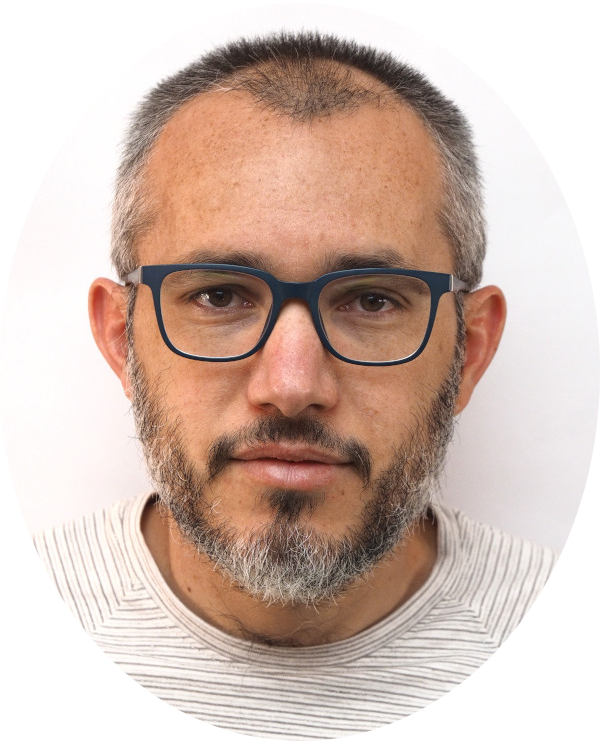
\includegraphics[width=.7\linewidth]{yo}
\end{center}

2$^a$ Privada Mapim\'i 610, Colonia Hip\'odromo\\
Durango, DGO\\
M\'exico\\[.2cm]
M\'ovil: \texttt{(+52) 618 116 82-37}\\
Whatsapp: \texttt{(+52) 618 116 82-37}\\
E-mail:
\begin{description}
	\item[Personal:] \href{mailto:gerardommc@gmail.com}{gerardommc@gmail.com}
	\item[Institucional:] \href{mailto:gerardo.mmc@enesmerida.unam.mx}{gerardo.mmc@enesmerida.unam.mx}
\end{description}
Born:  2 March 1981---Oxford, England\\
Nationality:  Mexicano

\end{multicols}

%%\hrule
\section*{Education}
\noindent

\years{2012-2017} \textsc{PhD} College of Public Health, Medical and Veterinary Sciences, James Cook University. Thesis:
\textbf{Modelling Hendra virus transmission from flying foxes to horses}.\\

\years{2007-2010}\textsc{MSc} in Conservation Biology, Instituto de Ecolog\'ia A.C. Thesis:
\textbf{A model of leptospirosis and comparison of its 
	frequency between two sites in the Perote ground squirrel (\emph{Spermophilus 
		perotensis}), and two domestic species}.\\

\years{2001-2006}\textsc{BSc} in Veterinary Medicine and Zootechnics, Universidad de LaSalle Baj\'io.\\

\years{2000-2001} 1st year Computer Science, Facultad de Matem\'aticas, Universidad de Guanajuato.\\

%%\hrule
\section*{Areas of specialisation}
Infectious disease ecology $ \bullet $ Publich Health $ \bullet $ Infectious disease modelling in wild animals $ \bullet $ Ecological niche modelling $ \bullet $ Spatial statistics $ \bullet $ Geographic information systems $ \bullet $ Conservation biology


\section*{Professional experience}

\years{2021-} Associate Lecturer, Escuela Nacional de Estudios Superiores unidad Mérida, Universidad Nacional Aut\'onoma de \'exico.

\years{2020} Pathology and Statistics Lecturer. Bachelor of Veterinary Sciences, Faculty of Veterinary Medicine and Zootechnics, Universidad Juárez del Estado de Durango. Durango, DGO. MX.

\years{2018-2020} Research associate. Ecological Health Research Group (\href{http://murraylab.weebly.com/}{Murray Lab}\footnote{\url{http://murraylab.weebly.com/}}),  Department of Infectious Disease Epidemiology, Faculty of Medicine, Imperial College London at St. Mary's.\\

\years{2017} External consultant. Project: \lq \lq Modeling Spillover\rq \rq (Defense Advanced Research Projects Agency, DARPA; D16AP00113), Bozeman Disease Ecology Lab, Montana State University.\\

\years{2012-2016} PhD student. \\

\years{2011-2012} Occasional field assistance for Dr. Mart\'in Pereda, Universidad Ju\'arez del Estado de Durango, Durango, DGO.\\

\years{2007} Private veterinary practice in small pet species.\\

\years{2006} Durrell Wildlife Conservation Trust, Jersey Zoo, Jersey, Channel Islands. Student placement. M.Sc. Javier L\'opez, head the Veterinary department. Research project: \lq \lq A pilot study on the anaesthtic effects of the combination of Ketamine – medetomidine, and propofol in the anuran \emph{Polypedates leucomystax}\rq \rq.\\

\years{2006} Animal Pathology Laboratory, Regional Cattle Union, Le\'on, Guanajuato, Mex. D.V.M. Manuel Conrado Gonz\'alez, head of the Pathology Laboratory. 600 h of professional social service. \\

%\hrule
\section*{Grants, honors \& awards}
\noindent

\years{2022-2023} Research project PAPIIT IA200822 \lq\lq Geostatistical estimation of ecological niches and applications in ecology, public health and conservation\rq\rq. \\

\years{2012-2016} Reseach grant of the National Hendra Virus Research Program, Australia. RIRDC PRJ-008213.\\

\years{2010} \emph{Bernardo Villa} award in the 1st Latin-American Congress of Mammalogy. First prize for academic excellence in the category MSc best thesis.\\

\section*{Publications \& talks}

\subsection*{Journal articles}
\noindent 

\years{2023} Eyal Goldstein, Joseph J. Erinjery, \textbf{Gerardo Mart\'in}, H. Janaka de Silva, Peter J. Diggle, David G. Lalloo, Kris A. Murray \& Takuya Iwamura. Climate change maladaptation for health: Agricultural practice against shifting seasonal precipitation affects snakebite risk for rural farmers in the tropics. \emph{iScience}. ISSN: 2589-0042 \url{https://doi.org/10.1016/j.isci.2023.105946}.\\

\years{2022} Jos\'e Mar\'ia Guti\'errez, Juliette Borri, Tamara Giles-Vernick, Romain Duda, Abdurazaq Habib, Anita Malhotra, \textbf{Gerardo Mart\'in}, Anna F. V. Pintor, Julien Potet, Terrence Scott, Isabelle Bolon, \& Rafael Ruiz Cata\~neda. Understanding and tackling snakebite envenoming with transdisciplinary research. \emph{PLoS Neglected Tropical Diseases}. ISSN: 1935-2735. \url{https://doi.org/10.1371/journal.pntd.0010897}. \\

\years{2022} \textbf{Gerardo Mart\'in}, Joseph J. Erinjery, Dileepa Ediriweera, David G. Lalloo, H. Janaka de Silva, Takuya Iwamura \& Kris A. Murray. A mechanistic model of snakebite as a zoonosis: envenoming incidence is driven by snake ecology, socioeconomics and its impacts on snakes. \emph{PLoS Neglected Tropical Diseases}. ISSN: 1935-2735. \url{http://dx.doi.org/10.1371/journal.pntd.0009867}.\\

\years{2022} \textbf{Gerardo Mart\'in}, Carlos Y\'a\~nez Arenas \& Xavier Chiappa Carrara. Discrepancies between point process models and environmental envelopes identify the niche centroid-geography configuration. \emph{Ecological Modelling}. ISSN: 0304-3800. \url{https://doi.org/10.1016/j.ecolmodel.2022.109974}.\\


\years{2021} \textbf{Gerardo Mar\'in}, Joseph Erinjery, Rikki Gumbs, Ruchira Somaweera, Dileepa Ediriweera, Peter J. Diggle, Anuradhani Kasturiratne, Janaka de Silva, David G. Lalloo, Takuya Iwamura \& Kris A. Murray. Integrating snake distribution, abundance and expert-derived behavioural traits predicts snakebite risk. \emph{Journal of Applied Ecology, En-prensa}.\\

\years{2021} \textbf{Gerardo Mar\'in}, Joseph Erinjery, Dileepa Ediriweera, David G. Lalloo, Takuya Iwamura \& Kris A. Murray. Redefining snakebite as a zoonosis: disease incidence is driven by snake ecology, socioeconomics and anthropogenic impacts. \emph{MedRXiv}. \url{https://doi.org/10.1101/2021.10.01.21264438}.\\

\years{2021} \textbf{Gerardo Martín}, Carlos Y\'a\~nez-Arenas, Rodrigo S. Camacho, Eyal Goldstein, Takuya Iwamura, Kris A. Murray \& Xavier Chiappa-Carrara. Effects of global environmental change on the burden of snakebite. \emph{ToxiconX}.\\

\years{2021} Eyal Goldstein,Joseph Erinjery, \textbf{Gerardo, Mart\'in}; Anuradhani Kasturiratne, Dileepa Ediriweera, Janaka de Silva, Peter J. Diggle, Peter, David G. Lalloo, Kris A. Murray, \& Takyua Iwamura. \textbf{Integrating human behavior and snake ecology with agent-based models to predict snakebite in high risk landscapes}. \emph{PLoS Neglected Tropical Diseases}.\\

\years{2020} Carlos Y\'a\~nez-Arenas, \textbf{Gerardo Mart\'in}, Luis Osorio-Olvera, Jazm\'in Escobar-Luj\'an, Sandra Casta\~no-Quintero \& Enrique Mart\'inez-Meyer. \textbf{The niche centrality hypothesis: key points about unfilled niches and the potential use of supraspecific modeling units}. \emph{Biodiversity Informatics}-\emph{en prensa}.\\

\years{2020} \textbf{Gerardo Mart\'in}, Mario Espinoza, Michelle Heupel, \& Colin Simpfendorfer (2020). \textbf{Estimating marine protected area network benefits for reef sharks}. \emph{Journal of Applied Ecology}. eISSN: 1365-2664. \url{https://doi.org/10.1111/1365-2664.13706}.\\

\years{2019} Kris Murray, \textbf{Gerardo Mart\'in} \& Takuya Iwamura (2019). \textbf{Focus on snake ecology to fight snakebite}. \emph{The Lancet}. (19) 325. ISSN: 01406736. \url{https://doi.org/10.1016/S0140-6736(19)32510-3}\\

\years{2018} \textbf{Mart\'in, Gerardo}; Becker, Daniel; Washburn, Alex \& Raina K. Plowright. \textbf{Environmental persistence of influenza H5N1 is driven by temperature and salinity: insights from a Bayesian meta-analysis}. \emph{Frontiers in Ecology and Evolution}.\\

\years{2018} Brannelly, Laura A.; \textbf{Mart\'in, Gerardo}; Lewellyn, John; Skerratt, Lee \& Lee Berger. \textbf{Size dependant susceptibility to chytridiomycosis in the invasive \emph{Rhinella marina}}. \emph{Diseases of Aquatic Organisms}.\\

\years{2018} \textbf{Mart\'in, Gerardo}; Y\'a\~nez-Arenas, Carlos; Plowright, Raina K.; Carla Chen \& Skerratt, Lee. \textbf{Hendra virus spillover is a bimodal system driven by climatic factors}. \emph{EcoHealth}.\\

\years{2018} \textbf{Mart\'in, Gerardo}; Y\'a\~nez-Arenas, Carlos; Plowright, Raina K.; Carla Chen \& Skerratt, Lee. \textbf{Climate change could increase the extent of areas at risk of Hendra virus spillover}. \emph{EcoHealth}.\\

\years{2017} Y\'a\~nez Arenas, Carlos Alberto; Rioja-Nieto, Rodolfo; Dzul-Manzanilla, Felipe; \textbf{Mart\'in, Gerardo}; Chiappa-Carrara, Xavier; Buenfil-\'Avila, Aura; Manrique-Saide, Pablo, Correa-Morales, Fabi\'an; D\'iaz-Qui\~n\'onez, Jos\'e Alberto; P\'erez-Renter\'ia, Crescencio; Ordo\~nez-\'Alvarez, Jos\'e \& Her\'on Huerta. \textbf{Characterization of environmental suitability for the Asian tiger mosquito (\emph{Aedes albopictus}) in M\'exico}. \emph{Journal of Medical Entomology}.\\

\years{2017} \textbf{Mart\'in, Gerardo}; Webb, Rebecca J.;Plowright, Raina K.; Chen, Carla  \& Lee F. Skerratt. \textbf{Microclimates might limit indirect spillover of the bat borne zoonotic Hendra virus}. \emph{Microbial ecology}.\\

\years{2016} \textbf{Mart\'in, Gerardo}; Skerratt, Lee; Y\'a\~nez-Arenas, Carlos; Plowright, Raina K. \& Carla Chen. \textbf{Climatic suitability influences species specific abundance patterns of Australian flying foxes and risk of Hendra virus spillover}. \emph{One Health Journal}.\\

\years{2016} Alison J. Peel, Hume E. Field, Peter A. Reid, Raina K. Plowright, Christopher C. Broder, Lee F. Skerratt, David T. S. Hayman, Olivier Restif, Melanie Taylor, \textbf{Gerardo Mart\'in}, Gary Crameri, Ina Smith, Michelle Baker, Glenn A. Marsh, Jennifer Barr, Andrew C. Breed, James L. N. Wood, Navneet Dhand, Jenny-Ann Toribio, Andrew A. Cunningham, Ian Fulton, Wayne L. Bryden, Cristy Secombe, Lin-Fa Wang, \textbf{The equine Hendra virus vaccine remains a highly effective preventative measure against infection in horses and humans: \lq The imperative to develop a human vaccine for the Hendra virus in Australia\rq\.} \emph{Infection Ecology and Epidemiology}. {6\bf}:31658.\\

\years{2015} \textbf{Mart\'in, Gerardo}; Plowright, Raina K.; Chen, Carla; Kault, David; Selleck, Paul \& Lee F. Skerratt. 2015. \textbf{Hendra virus survival does not explain the pattern of transmission and implicates relatively direct transmission routes}. \emph{Journal of General Virology}.\\

\years{2015} Plowright, Raina; Eby, Peggy; Hudson, Peter; Smith, Ina; Westcott, David; Bryden, Wayne; Middleton, Deborah; Reid, Peter; McFarlane, Rosemary; \textbf{Mart\'in, Gerardo}; Tabor, Gary; Skerratt, Lee; Anderson, Dale; Crameri, Gary; Quammen, David; Jordan, David; Freeman, Paul; Wang, Lin-Fa; Epstein, Jonathan; Marsh, Glenn; Kung, Nina \& Hamish McCallum. 2015. \textbf{Ecological Dynamics of Emerging Bat Virus Spillover}. \emph{Proceedings of the Royal Society B}.\\

\years{2013} Valdez-Lares, Rosaura; \textbf{Mart\'in-Mu\~noz de Cote, Gerardo A.}; Mu\~niz-Mart\'inez, Ra\'ul \& Georgina Santos-Barrera. \textbf{New distributional records for amphibians from Durango, M\'exico}. \emph{Herpetological Review}. 44 (4): 646-649.\\

\subsubsection*{In-review}

\years{2021} \textbf{Mart\'in, Gerardo}; Carlos Y\'a\~nez-Arenas \& Xavier Chiappa-Carrara. \textbf{Discrepancies between PPMs and MVEs identify the niche centroid - geography configuration}. \emph{Ecological Modelling}.

\subsubsection*{Ongoing projects}

\years{2019} Mart\'in, Gerardo \& Kris Murray. \textbf{Redefining snakebites as a zoonotic disease: implications for global change forecasting}.\\

\years{2019} Mart\'in, Gerardo \& Kris Murray. \textbf{Potential abundance of Sri Lankan venomous species}.\\

\years{2019} Mart\'in, Gerardo \& Kris Murray. \textbf{Predicting the impacts of global change on snakebite burden}.\\

\years{2018} Mart\'in, Gerardo; Webb, Rebecca J.; Plowright, Raina K.; Chen, Carla \& Lee F. Skerratt. \textbf{Tree cover in paddocks is the main determinant of exposure to Hendra virus in horses}.\\

\years{2018} Kosch, Tiffany \& Gerardo Mart\'in. \textbf{Modelling the prevalence of amphibian chytridiomycosis in Peru}.\\

\years{2018} Mart\'in, Gerardo; Giles, John R.; Westcott, David; Parry, Hazel; Plowright, Raina; Chen, Carla \& Lee F. Skerratt. \textbf{Landscape level mechanisms driving risk of Hendra virus spillover}.\\


\subsection*{Newspaper articles}
\noindent
\years{2013} Luly, Jon; Mart\'in, Gerardo; Skerratt, Lee. 30 April 2013. 
\textbf{Breaking up bat colonies doesn't eliminate health risks}. \emph{The 
Conversation} \footnote{\url{http://theconversation.com/breaking-up-bat-colonies-doesnt-eliminate-health-risks-13580}} \\


\subsection*{Talks \& poster presentation}

\years{2022} Congress of Production and Animal Health Sciences, Faculty of Veterinary Medicine and Zootechnics, UNAM, Mexico City. \emph{Ophidism and the ecology of zoonosis in light of global change}, keynote speech.\\

\years{2022} Mexican Scientific Congress of Ecology, Oaxaca, Oax.

\begin{enumerate}
	\item Oral presentation: \textbf{Identifying the geographic-environmental configuration of ecological niches}
	\item Poster: \textbf{Ophidism as a dynamic process during global change}
	\item Poster: \textbf{Agent based models to optimise reef shark protection in marine network protected areas}
\end{enumerate}

\years{2020} Institutional Seminar, Escuela Nacional de Estudios Superiores unidad Mérida. \textbf{Quantitative bridges between medicine and ecology}. \\

\years{2019} Association for Tropical Biology and Conservation, Asia-Pacific Chapter, Thulhiriya, Sri Lanka. \textbf{Abundance of venomous snakes of Sri Lanka in relation to climate and land cover}.\\

\years{2019} MRC winter seminar series, Imperial College London at St. Mary's. \textbf{The ecology of snakebite}.\\

\years{2017} Institutional seminar, Universidad de Guanajuato. \textbf{Ecology of infectious diseases: A chymera of biology?}.\\

\years{2017} Wildlife disease association 2017 International Conference, San Crist\'obal de las Casa, Chiapas, Mex. \textbf{Niche modelling studies on Hendra virus spillover ecology}. Talk.\\

\years{2017} Mathematics Colloquium Seminar, CIMAT, A. C. \textbf{Quantitative techniques to study the ecology of disease spillover}.\\

\years{2016} One Health Symposium. Division of Tropical Health and Medicine, College of Public Health, Medical and Veterinary Sciences, James Cook University. \textbf{Models that predict the risk of Hendra virus transmission from flying foxes to horses}. Talk.\\

\years{2016} CBMDT and CBTID, College of Public Health, Medical and Veterinary Sciences Fitzroy island retreat. \textbf{Models of Hendra virus survival to infer transmission pathways from bats to horses}. Talk.\\

\years{2016} CBMDT and CBTID, College of Public Health, Medical and Veterinary Sciences Fitzroy island retreat. \textbf{Models that predict risk of Hendra virus transmission from flying foxes to horses}. Poster.\\

\years{2015} Wildlife Disease Association 2015 International Conference, Maroochydore, QLD, Australia. \textbf{Understanding frequency of contact between
	horses and Hendra virus}. Poster.\\

\years{2014} Australasian Bat Society 2014 Conference. Townsville, QLD, Australia. \textbf{Hendra virus risk of spillover: The effect of weather and climate}. Talk.\\

\years{2013} Wildlife Diseases Association Australasian section 2013 Conference. Grampians, VIC, Australia. \textbf{Contribution of climate and weather to the distribution of Hendra virus spillover events}. Talk.\\

\years{2010} 10th National Congress of Mammalogy and 1st Latinamerican Congress of Mammalogy, Guanajuato, Gto., Mexico. \textbf{A model of leptospirosis and the comparisson of its frequency between two sites in the Perote ground squirrel (\emph{Xerospermophilus perotensis}) and two domestic species (\emph{Capra hircus} and \emph{Canis falimiaris})}. Talk.\\

\years{2009} 1st National Congress of Infectious Disease Ecology and Conservation Medicine , Veracruz, Ver., Mexico. \textbf{A model of leptospirosis and the comparisson of its frequency between two sites in the Perote ground squirrel (\emph{Spermophilus perotensis}) and two domestic species}. Talk.\\

\section*{Continuous education}

\years{2022} Formative evaluations for today's education. CUAIEED, UNAM.\\

\years{2018} Workshop. Software carpentry workshop: GIT and Linux shell. Imperial College London. South Kensington.\\

\years{2015} Workshop. Advanced tehcniques in data analysis with R. James Cook University, Townsville, QLD, AU. Lecturer: Murray Logan.\\

\years{2014} 2$^nd$ thematic schools \lq\lq Ecology, Evolution and Control of Infectious Diseases\rq\rq. Laboratory of Excellence CEBA, M\'erida, Ycat\'an. Lecturer: Dr. Jean Francois Gu\'egan.\\

\section*{General skills}
\begin{itemize}
\item Vehicle driving
\begin{itemize}
	\item Manual and automatic
	\item Wheel on left and right hand sides (Australian dirver's licence type \lq\lq O\rq\rq from Queensland)
	\item Small load vehicles
	\item Moderate experience with 4WD vehicles
\end{itemize}
\item Office: Libre/Open Office, MS Office, \TeX studio
\item Geographic information systems: R, Quantum GIS, SAGA
\item Scientific writing
\item Statistics with R: Spatial statistics, linear and non-linear regression, generalised linear models, generalised additive models, ecological niche modelling methods (Maxent, log-Gaussian fields, boosted regression trees, Poisson point process models), hypothesis tests.
\item MCMC sampling for Bayesian statistics with JAGS (similar to WinBUGS and OpenBUGS)
\item Field work
\begin{itemize}
	\item Small mammal trapping
	\item Camera trap sampling
	\item Animal tracking with GPS and radio emitters (limited experience)
\end{itemize}
\item Modelling and systems thinking with Stella
\item Image processing: The GIMP, Darktable
\item Programming languages (in exponentially decreasing order of experience):
\begin{itemize}
	\item R, \LaTeX, Python, Maxima
\end{itemize}	\item Image designa dn drawing: Inkscape, The GIMP
\item Linux for general purpose use, mainly Ubuntu and Debian based distributions
\end{itemize}


\section*{Languages}

{\sc Spanish}. Mother tongue\\
{\sc English}. Read, write and speak. IELTS score 7.0 (2010).\\

\section*{Other interests}

\begin{itemize}
	\item I've been playing classical guitar since 1998, although my first real lesson was in 2000 with Ju\'an M\'arquez and then with the great guitarist Juan Carlos Laguna.
	\item Wildlife photography
	\item Swimming
	\item Experimenting and trying linux distributions
\end{itemize}


%\hrule
\section*{Professional references}

Dr. Lee Skerratt\\
College of Public Health, Medical and Veterinary Sciences \\
James Cook University\\
Douglas, 4810 QLD, Australia\\
Phone: +61 7 4781 6065\\
Email: \href{mailto:lee.skerratt@jcu.edu.au}{lee.skerratt@jcu.edu.au}\\
\\
Dr. Alberto Gonz\'alez Romero\\
Departamento de Biolog\'ia y Conservaci\'on de Vertebrados \\
Instituto de Ecolog\'ia A. C.\\
Xalapa, Veracruz, M\'exico.\\
Phone: +52 228 842 1800 (ext) 4113\\
Email: \href{mailto:alberto.gonzalez@inecol.mx}{alberto.gonzalez@inecol.mx}\\
\\
Dr. Gerardo Suz\'an Azpiri\\
Facultad de Medicina Veterinaria y Zootecnia\\
Departamento de Etolog\'ia, Animales silvestres y de Laboratorio\\
Universidad Nacional Aut\'onoma de M\'exico\\
Distrito Federal, M\'exico\\
Phone: +52 555 622 5941 (ext) 5\\
Email: \href{mailto:gerardosuz@gmail.com}{gerardosuz@gmail.com}\\
\\
Dr. Carlos Y\'a\~nez-Arenas\\
Facultad de Ciencias, Parque Cient\'ifico y Tecnol\'ogico de Yucat\'an\\
Universidad Nacional Aut\'onoma de M\'exico\\
M\'erida, Yucat\'an, M\'exico\\
Phone: +52 999 406 0009 (ext) 7627\\
Email: \href{mailto:lichoso@gmail.com}{lichoso@gmail.com}\\
\\
Dr. Raina K. Plowright\\
Bozeman Disease Ecology Lab, Department of Immunology and Microbiology\\
Montana State University\\
Bozeman, MT, USA\\
Phone: +1 406 994 2939
Email:\href{mailto:rplowright@gmail.com}{rplowright@gmail.com} 
%\vspace{1cm}
\vfill{}
%\hrulefill
\begin{center}
{\scriptsize  Last updated: \today\- •\- 
% ---- PLEASE LEAVE THIS BACKLINK FOR ATTRIBUTION AS PER CC-LICENSE
Typeset in %\href{http://nitens.org/taraborelli/cvtex}{
%\fontspec{Times New Roman}
\XeTeX %}\\
% ---- FILL IN THE FULL URL TO YOUR CV HERE
%\href{http://nitens.org/taraborelli/cvtex}{http://nitens.org/taraborelli/cvtex}
}
\end{center}

\end{document}